%%%%%%%%%%%%%%%%%%%%%%% file typeinst.tex %%%%%%%%%%%%%%%%%%%%%%%%%
%
% This is the LaTeX source for the instructions to authors using
% the LaTeX document class 'llncs.cls' for contributions to
% the Lecture Notes in Computer Sciences series.
% http://www.springer.com/lncs       Springer Heidelberg 2006/05/04
%
% It may be used as a template for your own input - copy it
% to a new file with a new name and use it as the basis
% for your article.
%
% NB: the document class 'llncs' has its own and detailed documentation, see
% ftp://ftp.springer.de/data/pubftp/pub/tex/latex/llncs/latex2e/llncsdoc.pdf
%
%%%%%%%%%%%%%%%%%%%%%%%%%%%%%%%%%%%%%%%%%%%%%%%%%%%%%%%%%%%%%%%%%%%


%\documentclass[runningheads,a4paper]{llncs}
\documentclass[envcountreset,oribibl]{llncs}

\usepackage{amssymb}
\setcounter{tocdepth}{3}
\usepackage{graphicx}
\usepackage{amsmath}
\usepackage{comment}
\usepackage{bm}
\usepackage[lined,boxed,commentsnumbered, ruled]{algorithm2e}
\usepackage{algorithmic}
\usepackage{indentfirst}
\usepackage{multirow}


\usepackage{url}
\urldef{\mailsa}\path|{alfred.hofmann, ursula.barth, ingrid.haas, frank.holzwarth,|
\urldef{\mailsb}\path|anna.kramer, leonie.kunz, christine.reiss, nicole.sator,|
\urldef{\mailsc}\path|erika.siebert-cole, peter.strasser, lncs}@springer.com|
\newcommand{\keywords}[1]{\par\addvspace\baselineskip
\noindent\keywordname\enspace\ignorespaces#1}
\newtheorem{defn}{Definition}

\begin{document}
\bibliographystyle{plain}

\mainmatter  % start of an individual contribution

% first the title is needed
\title{OPGs-Rec: Organized-POI-Groups Based Recommendation}

% a short form should be given in case it is too long for the running head
\titlerunning{OPGs-Rec: Organized-POI-Groups Based Recommendation}

% the name(s) of the author(s) follow(s) next
%
% NB: Chinese authors should write their first names(s) in front of
% their surnames. This ensures that the names appear correctly in
% the running heads and the author index.
%
\author{JiaPeng Li$^{1}$, Yanxia Xu$^{1}$, Lei Zhao$^{1}$}
%
\authorrunning{J. Li et al.}

\institute{$^1$School of Computer Science and Technology, Soochow University China\\
\email{trajepl@gmail.com, xyx.edu@gmail.com, zhaol@suda.edu.cn}\\
}

%
% NB: a more complex sample for affiliations and the mapping to the
% corresponding authors can be found in the file "llncs.dem"
% (search for the string "\mainmatter" where a contribution starts).
% "llncs.dem" accompanies the document class "llncs.cls".
%

\toctitle{Lecture Notes in Computer Science}
\tocauthor{Authors' Instructions}
\maketitle


\begin{abstract}
With development of urban modernization, a large number of Organized POI Groups(OPGs), such as multipurpose buildings, business streets and shopping malls, scatter over the city which have a great impact on people's lives and urban planning etc. Nowadays recommender system is based on Point-of-Interest(POI) which plays an important role in ours lives. However, it is well-known that there exists no work about groups of POIs which serves in recommendation. In this paper, we propose an OPGs-Rec, a novel OPGs-Based recommender system that recommends OPGs extracted from sets of POIs to target users by their locations and needs. We will demonstrate step by step how use OPGs to recommend valuable information to target users.
\keywords{OPGs recommendation; Organized POI groups; Density-based Clustering}
\end{abstract}

\section{Introduction}
With the proliferation of spatial data, lots of research work on spatial recommendation has been presented. The development of urban modernization fosters a large number of hot spots, such as multipurpose buildings, business streets and shopping malls. One of these hot spots is larger than a single POI and smaller than a functional region\cite{Yuan12}. Intuitively, a large hot spot is defined as Oganized POIs Group(OPG)\cite{Xu15} has a set of POIs which locate close to each other. The OPGs not only reflect the distribution of the center of city, but also have a great effect on recommendation. If an user plans a series of activities(e.g., shopping, watching a movie or having dinner), the existing POIs-Based recommendation usually recommend the best POI according to evaluation functions. Users will receive a set of nearest POIs which cover all of user's requirements\cite{Cao11} or a set of related POIs with higher ranking\cite{Chen15}. However, people have their individual requirements and the existing POIs-Based recommendation cannot meet all of people's requirements simultaneously. Besides, an enormous number of people are unclear about their requirements until they have a visit to the POI recommended. For example, a woman plans to buy a pair of shoes. But she is unclear about what kind of shoes she wants until she has a shopping. There are also so many other possibilities after buying a pair of shoes, Maybe she suddenly wants to buy a skirt to match her new shoes. Obviously, the OPGs-Based recommendation can offer user more choices than traditional POIs-Based recommendation. Hence, recommending a shopping mall flexibly is better than recommending several shoes shops according to evaluation functions because the users can choose the best one just taking a little time.

To recommend a set of Organized POIs Groups, this paper proposes a novel system OPGs-Based Recommender System(OPGs-Rec). It will be shown that when an user plans a series of activities, recommendation based OPGs is more efficient and the accuracy does not obviously decrease. The solution to discovering OPGs from lots of POIs is a variant of density-based clustering algorithm, i.e. DBSCAN\cite{Xu15}. After clustering POIs, we get a complete file \textit{R} which contains a set of OPGs $O=<O_1, O_2, O_3...O_n>$. Each OPG contains a set of POIs which locate close to each other, i.e. $O_i=<P_1, P_2, P_3...P_n>$. There is $P_i=<LOG, LAT, M, L, I>$ which indicates geographical longitude, geographical latitude, address of POI, tags of POI and ID of OPGs in order. For these sets of $P_i$, we extract the name information of OPGs from sets of $P_i.M$ which group by value of $P_i.I$ for further recommendation.


\begin{figure}
   \centering
    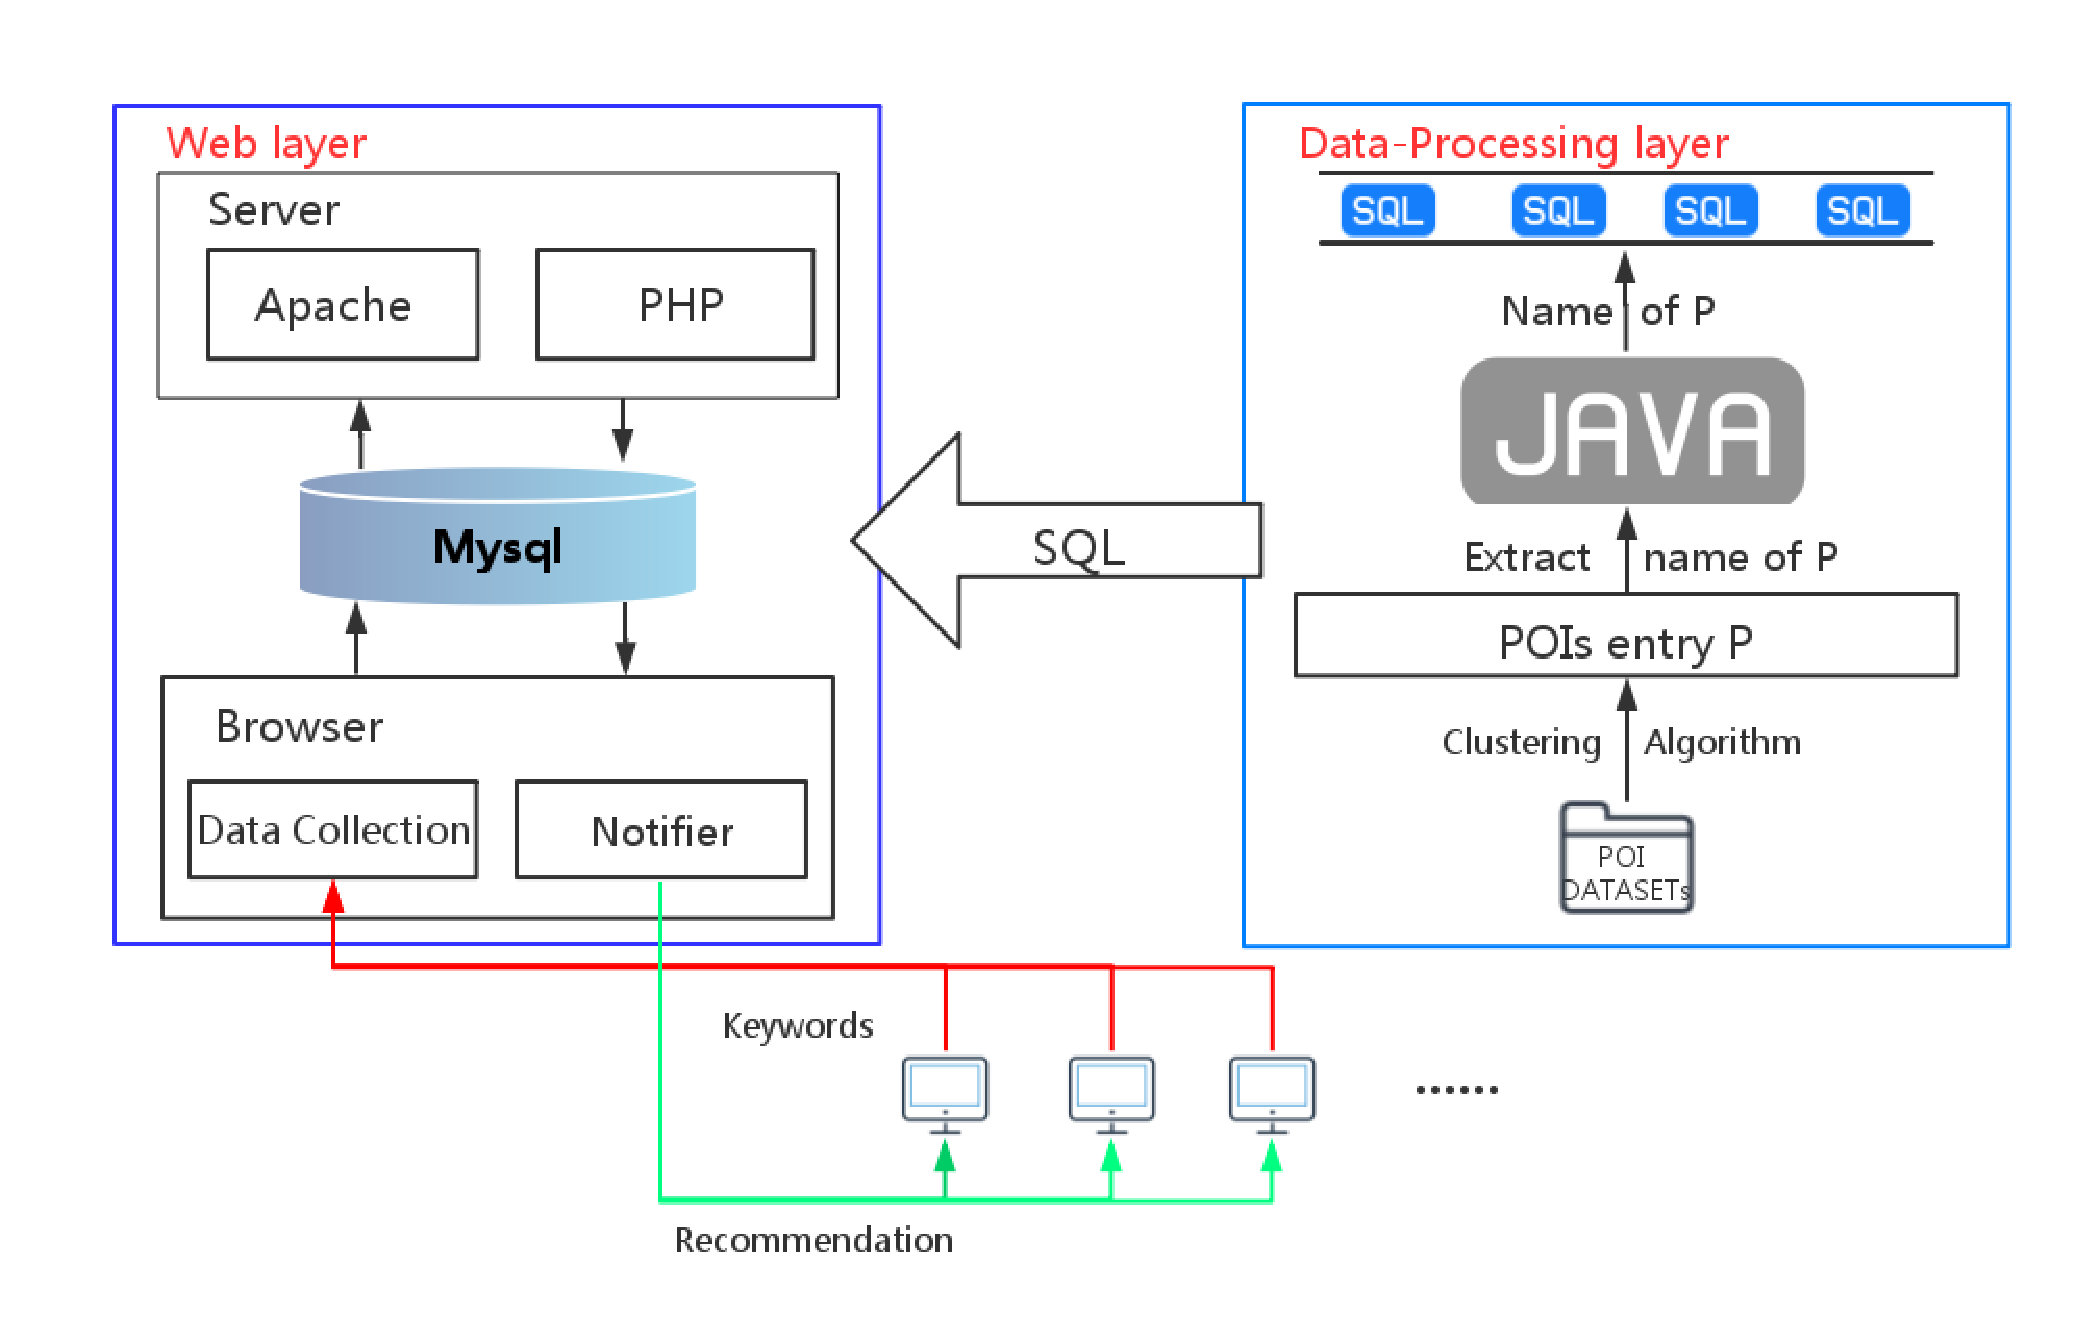
\includegraphics [width=0.75\textwidth] {pics/System.pdf}
\caption{System overview}
\label{fig:reputation}
\end{figure}


\section{System Overview} \label{sec:model}
As shown in Figure 1, our recommender system OPGs-Rec has two layers: Web architecture layer and Data-Processing layer. The front-end of our recommender system is designed with a good interaction and presentation. The backstage of OPGs-Rec provides an interface for interacting with Mysql storing a series of dataset that processed by Data-Processing layer. Each party has several components and their functionalities are described as follows.

\textbf{Web layer:}
The front end of website is designed with a good interaction and presentation. As you can see, in Figure 2, there are three regions forming our page: keyword-select, result table and the map display. When you visit our page, you can delimit the scope with a circle when you click the button is at upper right corner. Then you can select the keywords got from google POI classification\footnote{http://lbs.juhe.cn/data.php?PHPSESSID=acunetixsessionfixation} in keyword-select region. Finally, the backstage returns OPGs related all keywords you input. The feedback results are shown ordered by the linear addition of distance from circle center and the evaluation ranking. Note that, if you do not delimit the scope, this page will raise a warning. 

Generally, the data entry $IN = (L, R, K)$ created in font-end is considered as input data of our recommendation. $IN.L$ and $IN.R$ is the center and radius of circle. $IN.K$ is the keywords that users can select. The output data depends on these three elements is represented as the $OUT=(ID, Info)$ indicates the ID and information of OPGs. Every OPG in $OUT$ is displayed as a covering in the map.The audience could act as users and visit our website in http://ada.suda.edu.cn/opg/. 

\textbf{Data Processing layer:}
In this layer, we process the original POIs dataset using a variant of density-based clustering algorithms i.e. DBSCAN using hybrid similarity which different from traditional DBSCAN.(The details can be seen in \cite{Xu15}.) In this way, we can get a set of OPGs $O = (O_1, O_2, O_3... O_n)$ mentioned above. Then we we extract the name information of OPGs. As you can see, in Figure3, there are 701 OPGs clustered from original POIs dataset.

\textbf{System Implementation:} The Web layer is implemented as a B/S pattern based on Apache2.4, php7 and Baidu Map API\footnote{http://developer.baidu.com/map/reference/index.php}. For Data-Processing layer, we use OpenJDK8 Runtime Environment and OpenJDK 64-Bit Server VM to processing POIs dataset and output sql file to insert keywords and some supplementary information to Mysql. The version of Mysql is Ver 15.1 Distrib 10.1.12-MariaDB, for Linux (x86-64).

\begin{figure}
	\begin{minipage}[t]{0.5\linewidth}
		\centering
		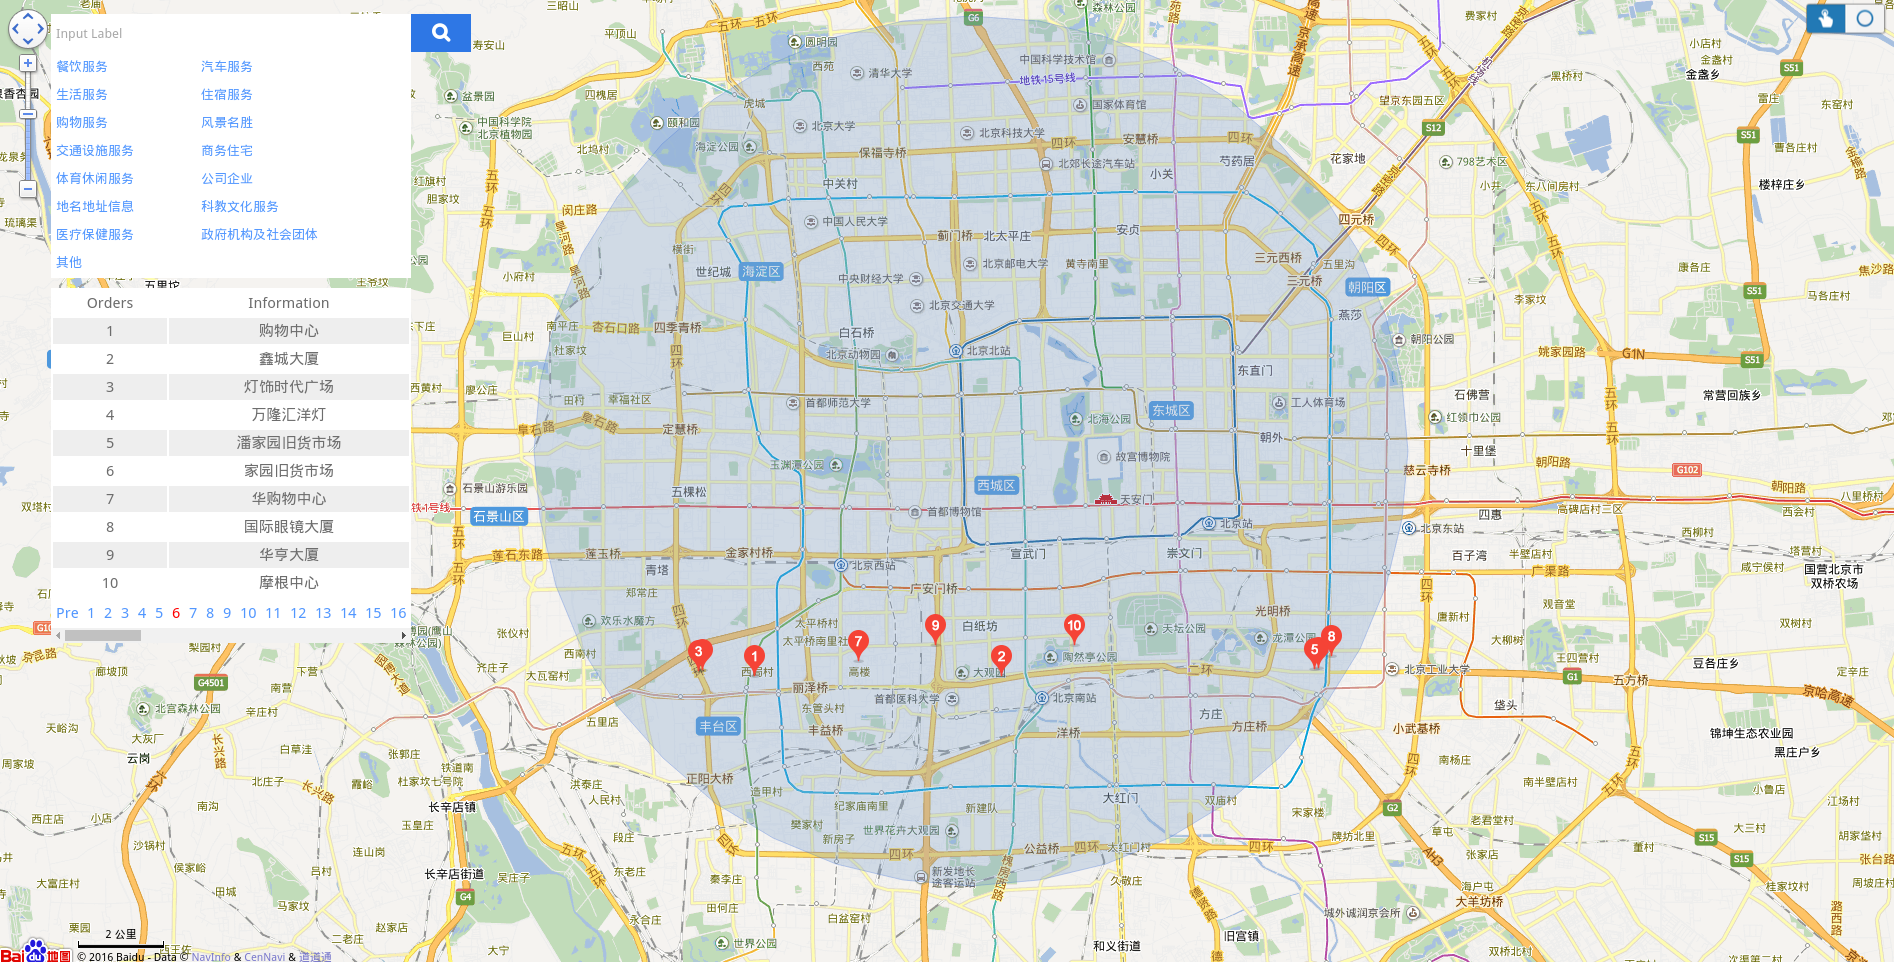
\includegraphics[height = 3cm, width = 6cm]{pics/classify.png}
		\caption{OPGs classify}
		\label{fig:1}
	\end{minipage}
	\begin{minipage}[t]{0.5\linewidth}
		\centering
		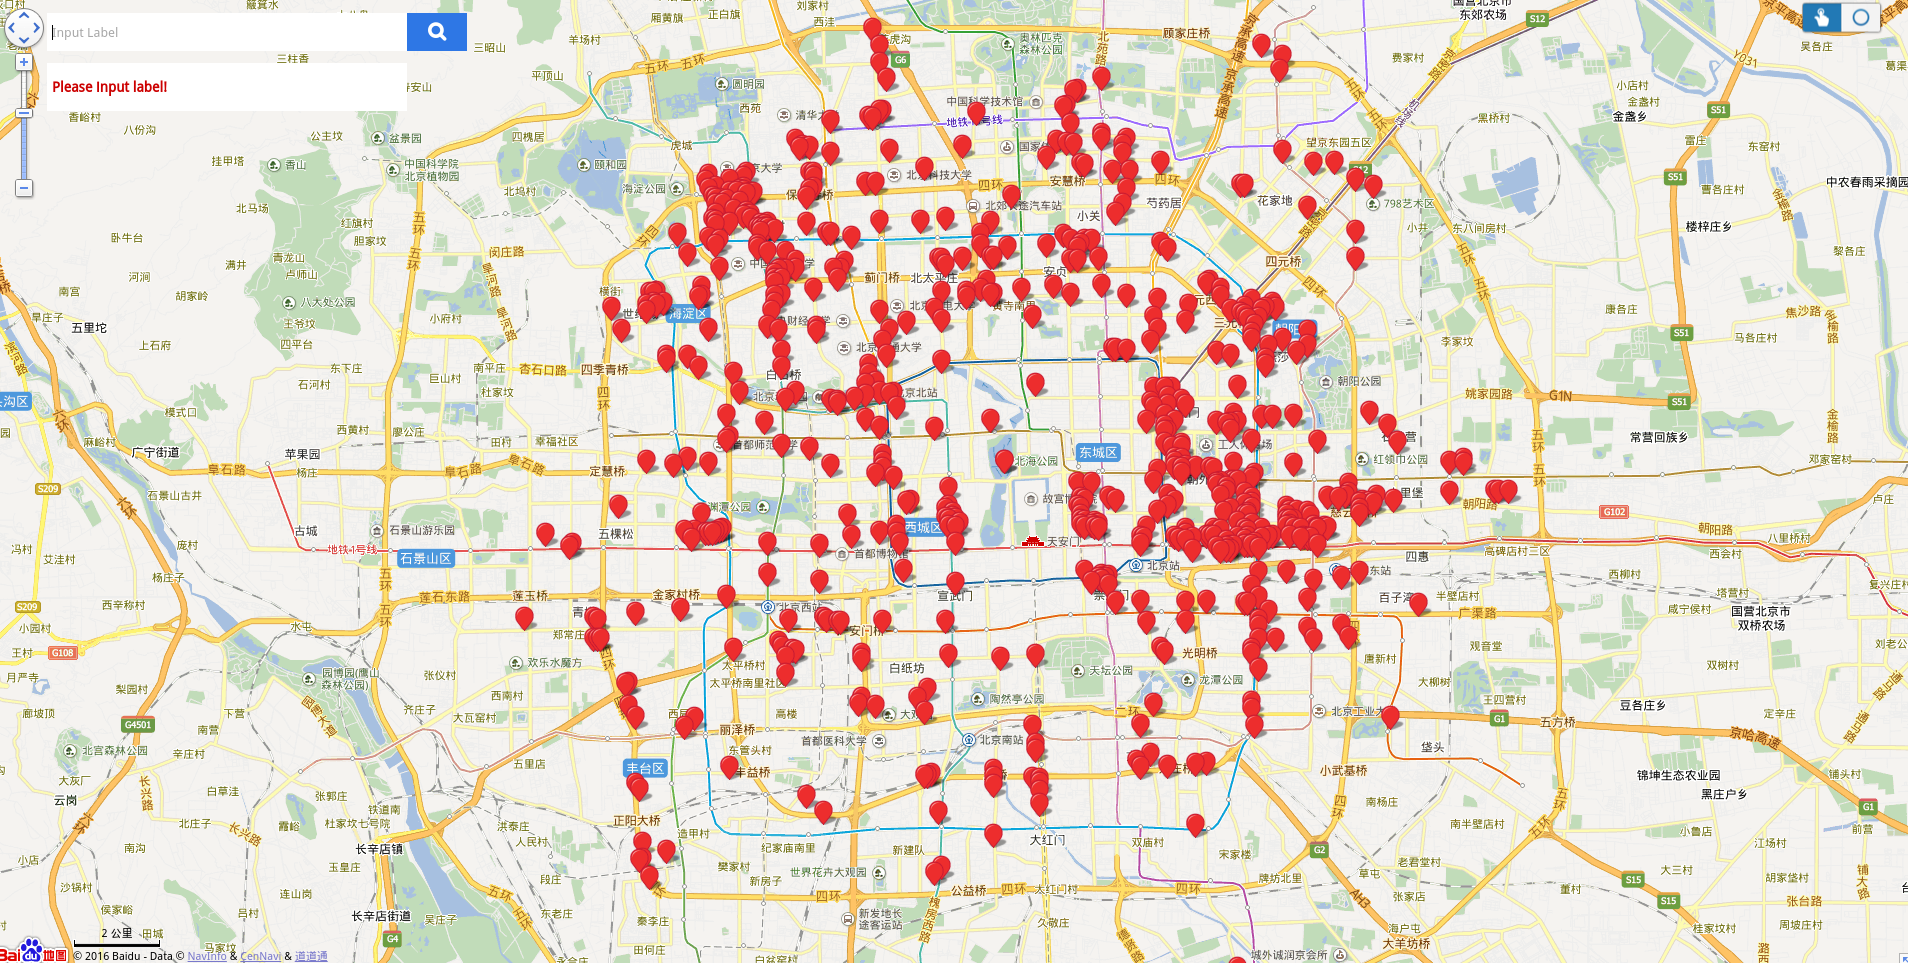
\includegraphics[height = 3cm, width = 6cm]{pics/OPGs.png}
		\caption{All OPGs in Beijing 2014}
		\label{fig:1}
	\end{minipage}
\end{figure}

\begin{figure}
	\begin{minipage}[t]{0.5\linewidth}
		\centering
		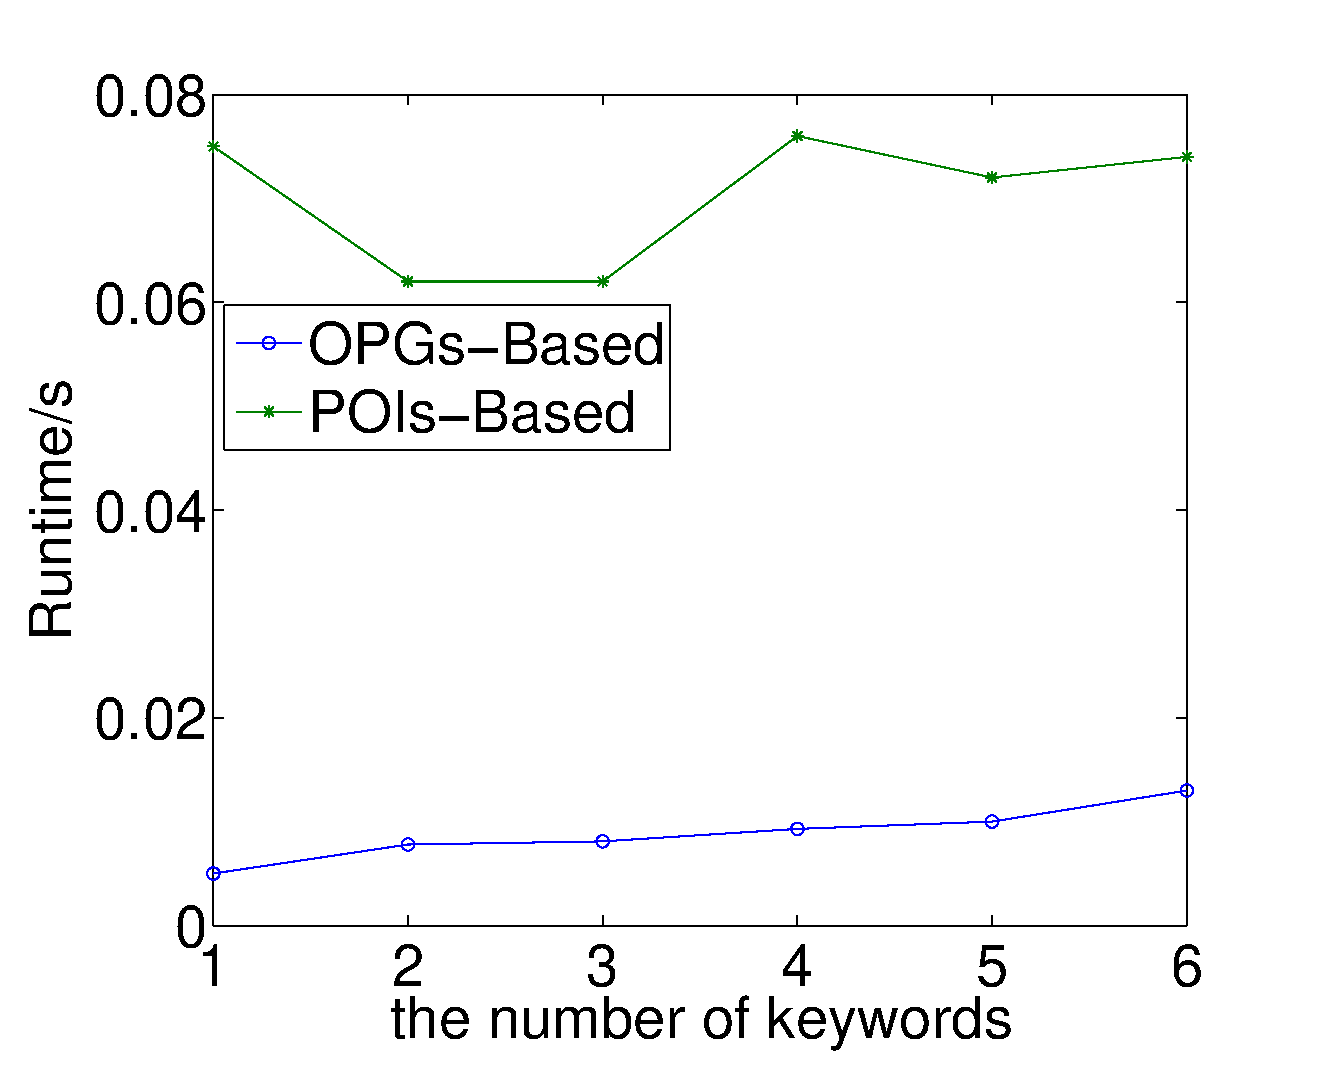
\includegraphics[width=5cm, height = 3.8cm]{pics/figure1.eps}
		\caption{Efficiency}
		\label{fig:1}
	\end{minipage}
	\begin{minipage}[t]{0.5\linewidth}
		\centering
		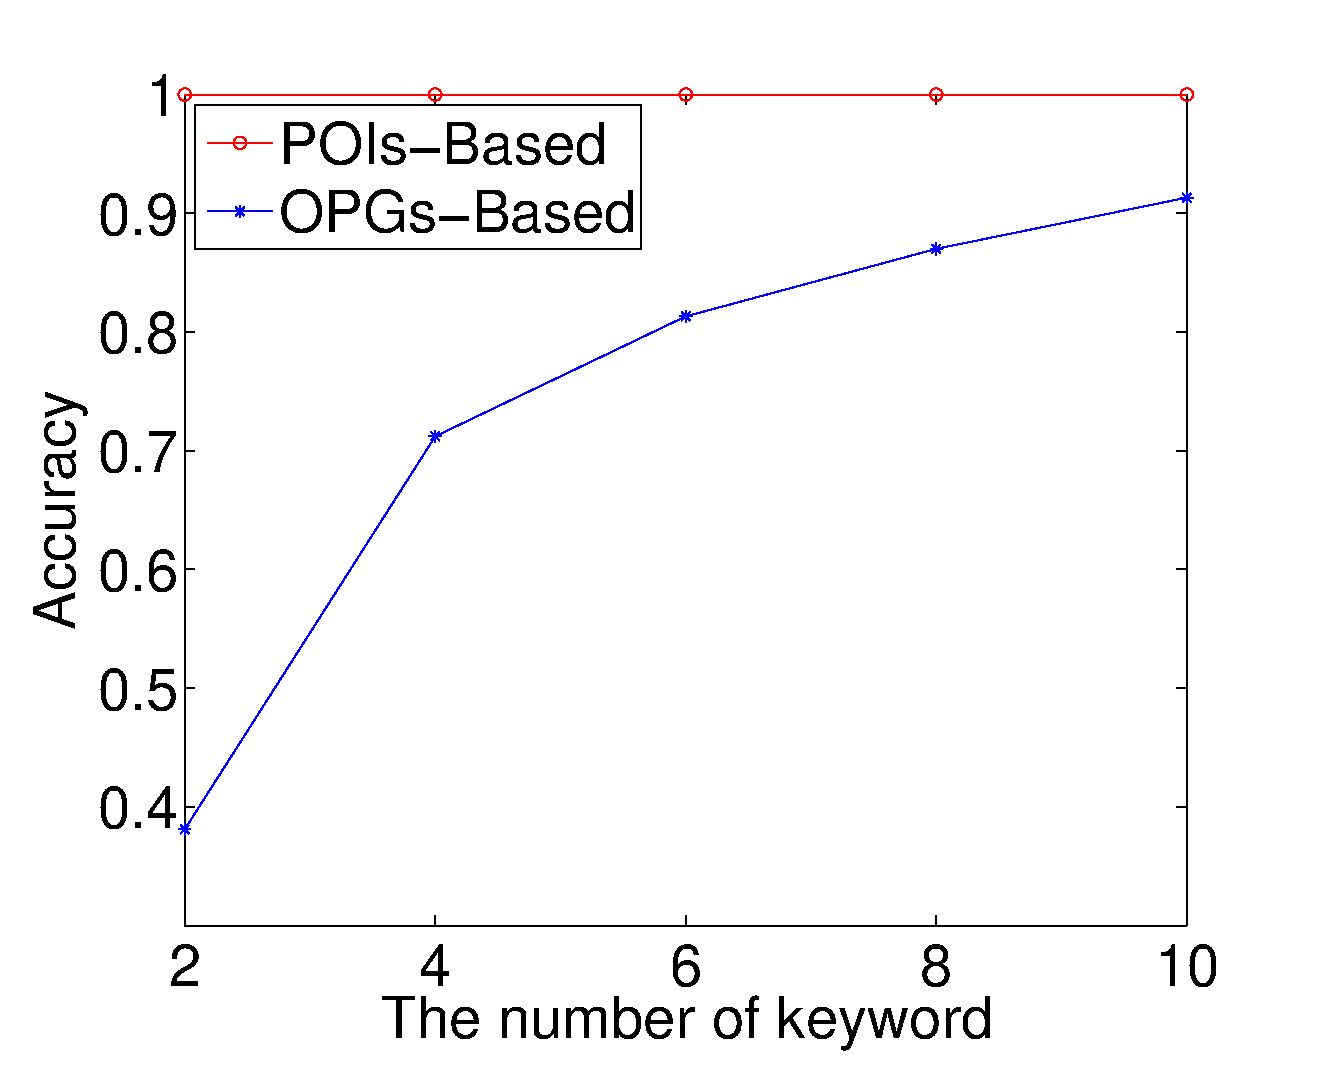
\includegraphics[width=5cm, height = 3.8cm]{pics/figure3.eps}
		\caption{Accuracy}
		\label{fig:1}
	\end{minipage}
\end{figure}


\section{Performance}\label{sec:demon}
This section, we conduct experiment using the POIs data in Beijing(2014) which has 490317 POIs. We process this dataset getting 701 OPGs stored in Mysql. Figure 4 shows that the different running time of OPGs-Rec and POIs-based when there are different numbers of keywords.  As you can see, the OPGs-Rec is more efficient than POIs-Based recommendation. In Figure 5, with the increasing of keywords, the accuracy of OPGs-Rec increases obviously. In table 1, it shows the number of POIs and OPGs that recommended depending on different distances from location of users. The OPGs-Rec greatly increases efficiency and accuracy of recommendation obviously. When an user plans a series of activities, he can find all he wants in several OPGs quickly and accurately.
\begin{table}[!h]
	\centering
	\caption{POI and OPGs search results}
	\label{number of sub-tra}
	\begin{small}
		\begin{tabular}{p{1cm}|p{1.5cm}|p{1.5cm}|p{1.5cm}|p{1.5cm}|p{1.5cm}|p{1.5cm}}
			\hline
			 & 500m & 1000m & 1500m & 2000m &2500m & 3000m\\ \hline
			POI & 2318 & 5399 & 9080 & 14281 & 19226 & 21575 \\\hline
			OPG & 2 & 3 & 3 & 7 & 7 & 7\\\hline
		\end{tabular}
	\end{small}
\end{table}
 
\begin{thebibliography}{4}

\bibitem{Yuan12}
Jing Yuan, Yu Zheng, Xing Xie: Discovering regions of different functions in a city using human mobility and POIs. KDD 2012: 186-194

\bibitem{Xu15}
Yanxia Xu, Guanfeng Liu, Hongzhi Yin, Jiajie Xu, Kai Zheng, Lei Zhao: Discovering Organized POI Groups in a City. DASFAA Workshops 2015: 223-226

\bibitem{Cao11}
Xin Cao, Gao Cong, Christian S. Jensen, Beng Chin Ooi: Collective spatial keyword querying. SIGMOD Conference 2011: 373-384

\bibitem{Chen15}
Wei Chen, Lei Zhao, Jiajie Xu, Guanfeng Liu, Kai Zheng, Xiaofang Zhou: Trip Oriented Search on Activity Trajectory. J. Comput. Sci. Technol. 30(4): 745-761 (2015)

\end{thebibliography}

\end{document}
